\section{Une étude de cas : Cholesky}\label{chap:contribs:apps:cholesky}

Afin de mettre en application nos analyses nous avons choisi comme cas d'étude une application d'algèbre linéaire populaire et bien connue : la factorisation de Cholesky.
Une manière standard de paralléliser les applications d'algèbre linéaire est de découper le problème en l'appliquant à différentes sous parties (ou \emph{blocs}) des matrices.

Nous allons étudier en détails l'algorithme de Cholesky par bloc, voir quelles sont ses parties critiques et leurs comportements, et nous allons également voir comment nous avons pu améliorer son exécution.


\subsection{Description générale}

La factorisation de Cholesky a pour but de résoudre l'équation suivante :

$$ A = L*L^T$$

Où $A$ est une matrice symétrique définie positive de nombre réels, et $L$ est l'inconnue, une matrice triangulaire inférieure.

Pour paralléliser la résolution de cette équation, on va découper la matrice $A$ par bloc, et appliquer un algorithme de Cholesky par bloc.
On peut donc caractériser une factorisation de Cholesky par sa taille de bloc et sa largeur en nombre de blocs.

L'algorithme de résolution par bloc repose sur quatre algorithmes basiques d'algèbre linéaire tirés des \emph{BLAS} - \emph{Basic Linear Algebra Subprograms} - décrit ci-dessous~:


\paragraph{POTRF(A)}

Ce noyau effectue la factorisation de Cholesky de base sur une matrice $A$.

\paragraph{TRSM(A, B)}

Ce noyau effectue l'opération suivante~: $A*X = B$, où $A$ est une matrice triangulaire, et $B$ une matrice générique. $B$ est écrasée par la matrice solution $X$.

\paragraph{SYRK(A, C)}

Ce noyau effectue l'opération suivante~: $C = A*A' + C$, où $A$ est une matrice générique, et $C$ est une matrice symétrique.

\paragraph{GEMM(A, B, C)}

Ce noyau effectue une multiplication de matrices génériques, définie de la manière suivante~: $C = A*B + C$, où $A$, $B$, et $C$ sont des matrices génériques.

L'algorithme peut se formuler de la manière suivante~:

\begin{lstlisting}[language=c++]
for (int k = 0; k < n_blocs; k++) {
  DPOTRF(A(k, k));

  for (int m = k+1; m < n_blocs; m++) {
    DTRSM(A(k, k), A(k, m));

    for (int m = k+1; m < n_blocs; m++) {
      DSYRK(A(k, m), A(k, k));

      for (int n = k+1; n < m; n++) {
        DGEMM(A(k, n), A(k, m), A(n, m));
      }
    }
  }
}
\end{lstlisting}

Pour mieux imager l'algorithme, les opérations se produisant sur chaque bloc de la matrice au rang |k| sont illustrées sur la figure~\ref{fig:contribs:apps:cholesky:rank-update}

\begin{figure}[ht]
  \centering
  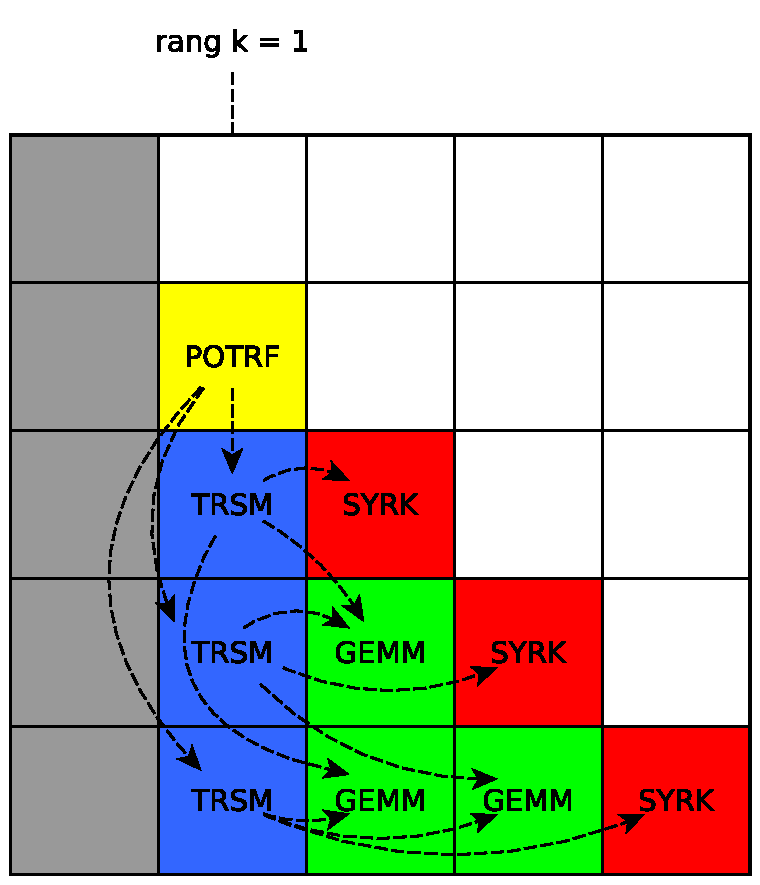
\includegraphics[width=0.6\textwidth]{cholesky-rank-update}
  \caption{Itération du rang k de la factorisation de Cholesky}\label{fig:contribs:apps:cholesky:rank-update}
\end{figure}


\subsection{Graphe de dépendances}

\begin{figure}[ht]
  \centering
  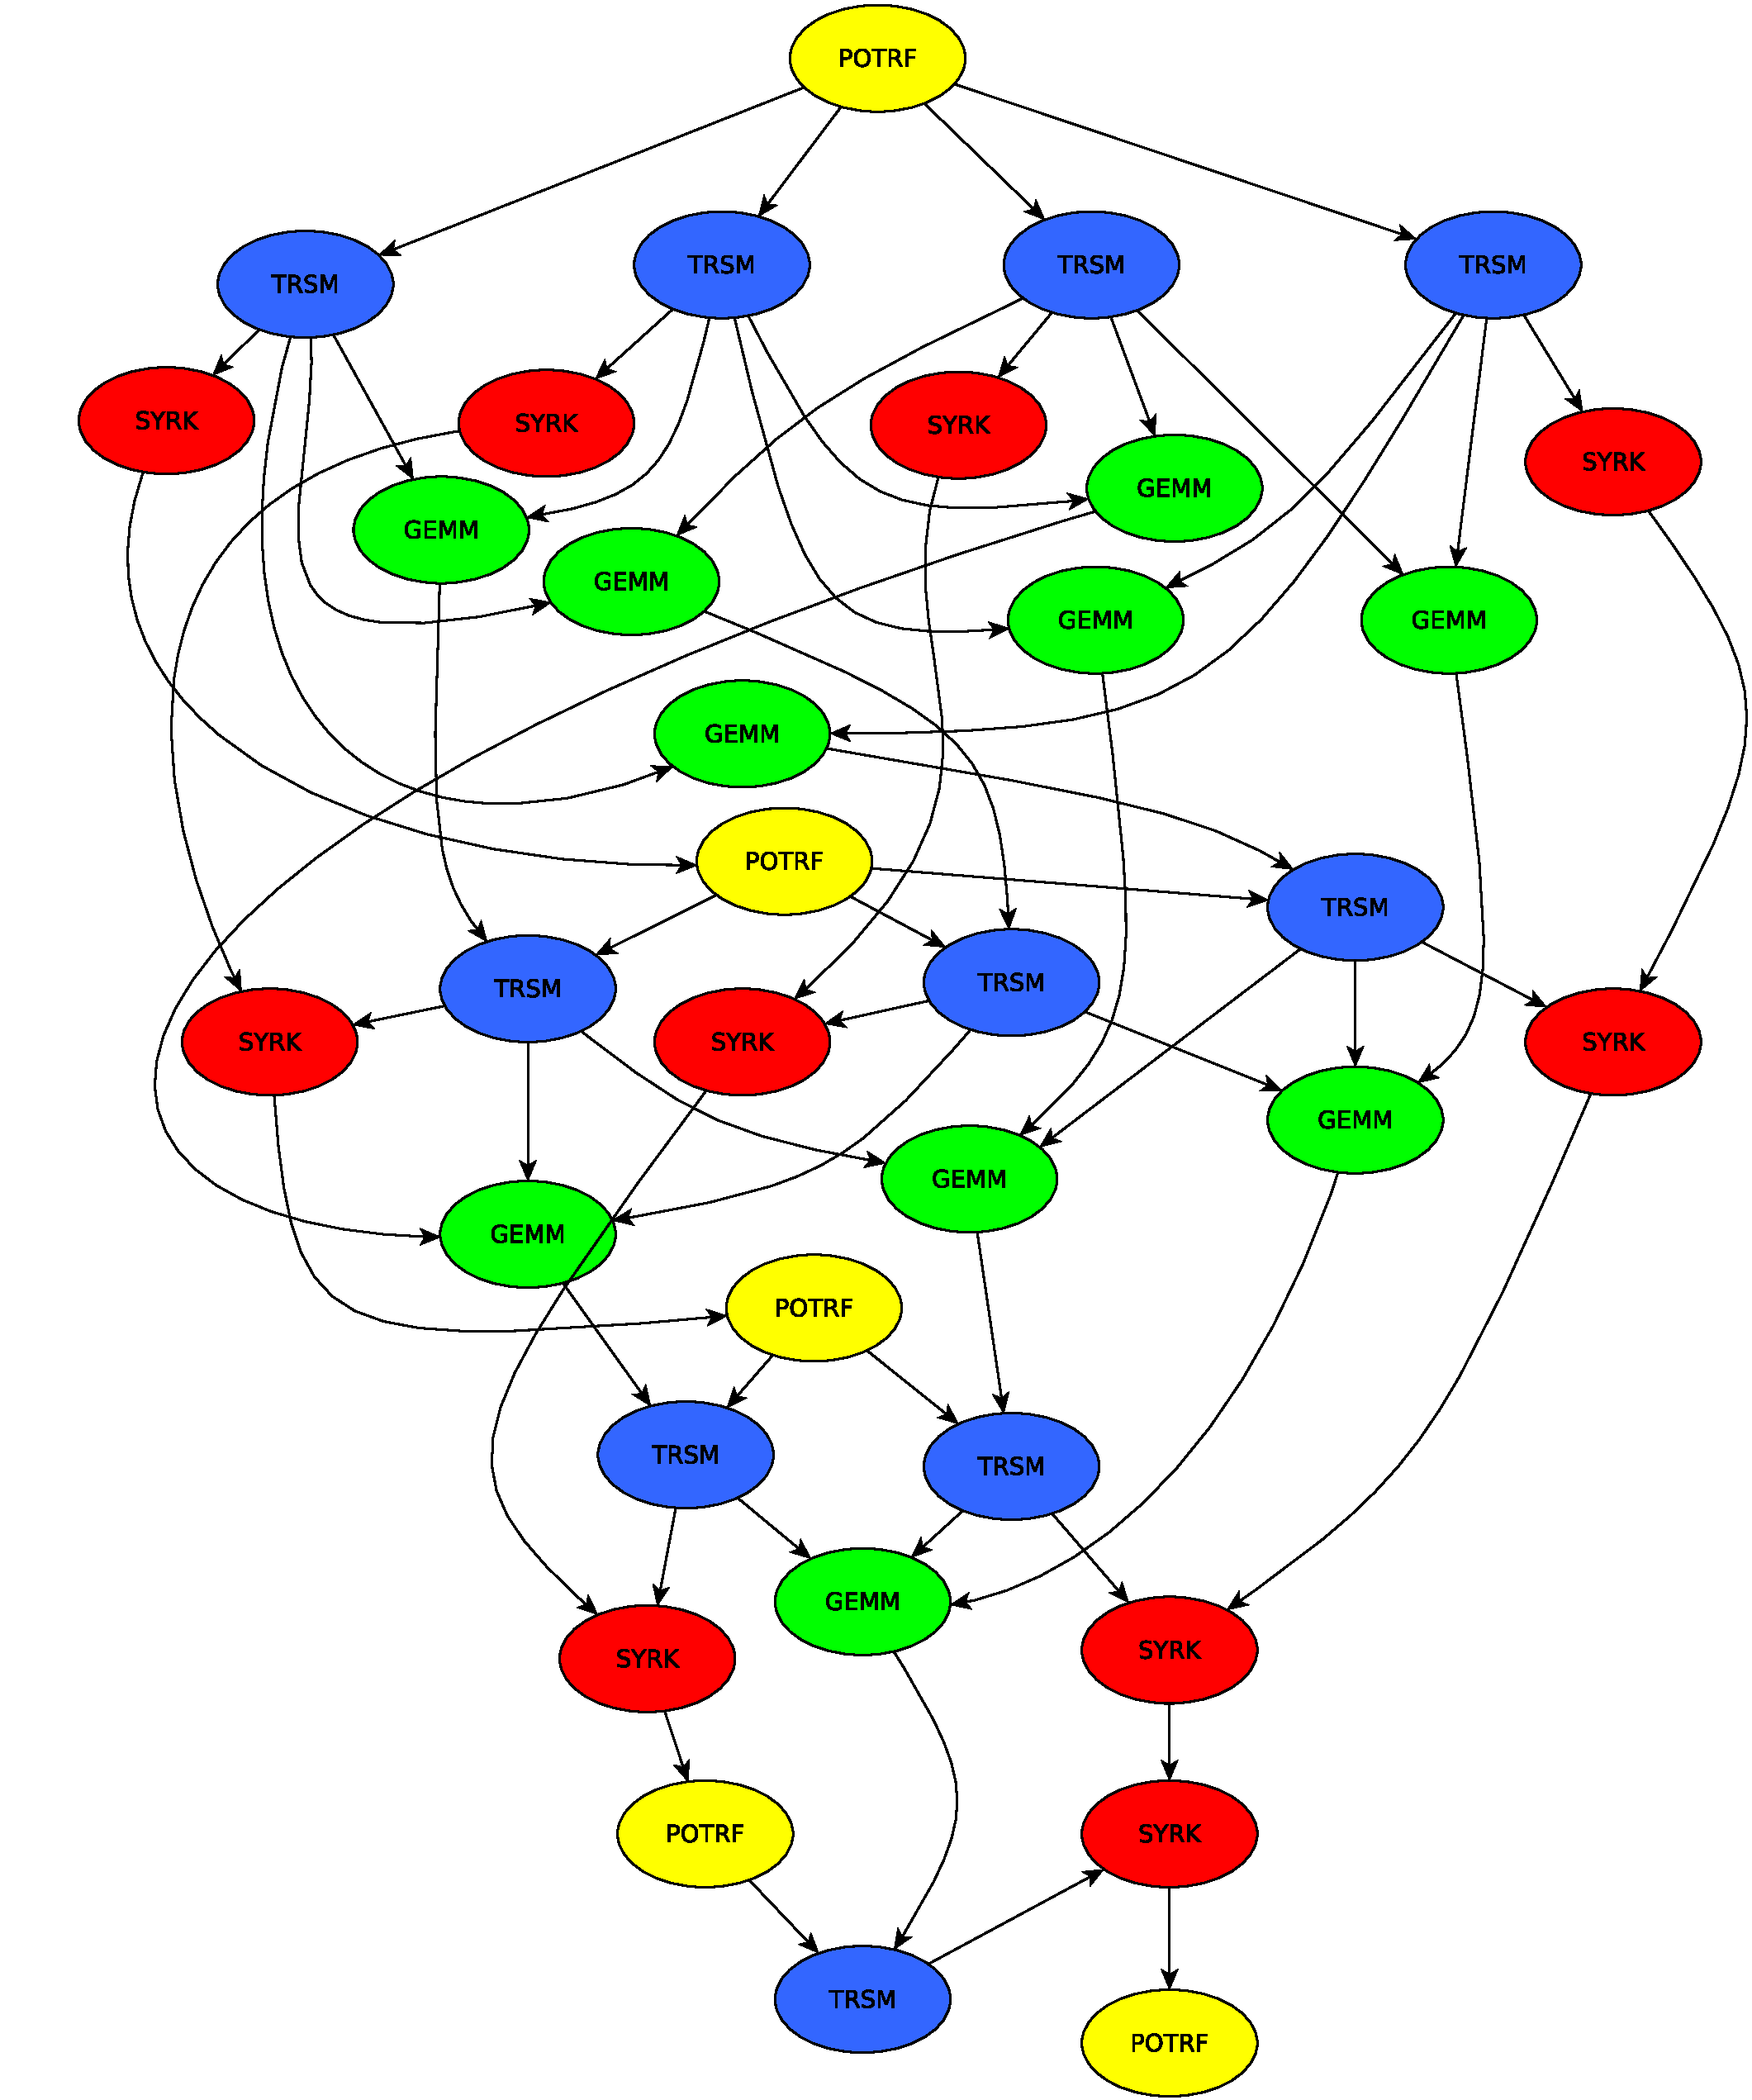
\includegraphics[width=0.7\textwidth]{cholesky-dag-5}
  \caption{DAG d'un Cholesky de largeur 5}\label{fig:contribs:apps:cholesky:dag-5}
\end{figure}


Décrire aussi dépendances de chaque tâche


maj des sous matrices diagonales restantes

TODO : décrire en détail l'algorithme de Cholesky, et faire un point sur les différentes performances que l'on obtient en fonction de comment on fait varier l'initialisation de données.

GRAPHE : 4.2.4 schéma du DAG de Cholesky, un joli graph en couleur avec une couleur par noyau. point bonus pour un schéma explicatif du fait que dpotrf est la clé pour générer le parallélisme.

GRAPHE : 4.2.4 performances détaillées Cholesky : impact de la taille de la matrice, de la taille de bloc, de la machine. tailles = 8k, 16k, 32k, bs = 128/256/512. (*sans* affinité, juste un topo)

